\section{Part 1}

\subsection{Converting given formula \texttt{F} to 3COL graph}

As the first letter of my first name begins with a \textit{D}, I will be working with the following formula

\begin{equation}\label{eq:original-formula}
F = (z_1 \lor z_2) \land (z_1 \lor z_2 \lor z_3 \lor z_4) 
\end{equation}

To convert this to 3COL I first needed to covert the formula into 3SAT. The conversion to 3SAT looks like the following

\begin{equation}\label{eq:original-formula}
F = (z_1 \lor z_2 \lor Y_1) \land (\overline{Y_1} \lor z_1 \lor z_2) \land (z_1 \lor z_2 \lor Y_2) \land(\overline{Y_2} \lor z_3 \lor z_4)
\end{equation}

The resulting 3COL graph can be seen in the image below

\begin{figure}[h!]
\vspace{-5pt}
\centering
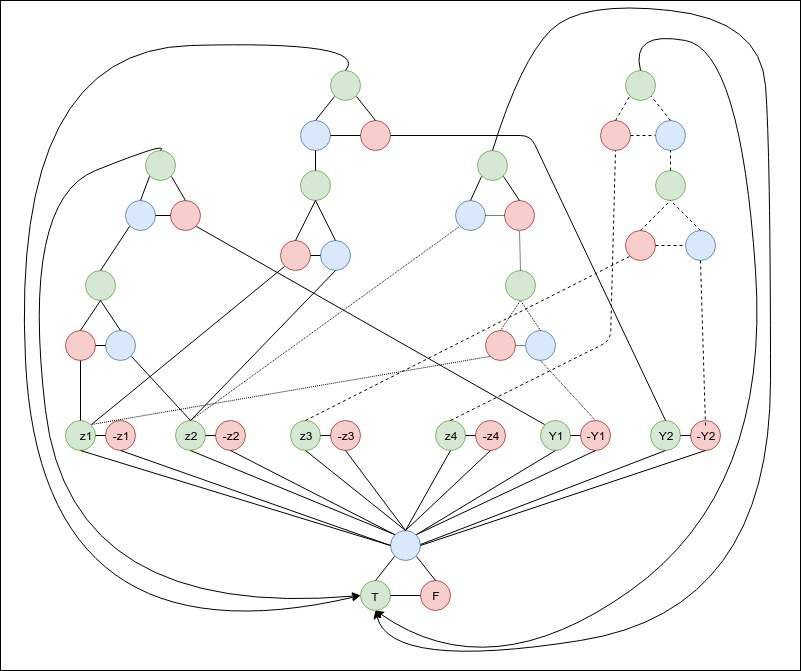
\includegraphics[width=1.0\textwidth]{images/3col.jpg}
\caption{\label{fig:3col_graph}3COL graph}
\end{figure}